\chapter{System Architecture}
In this thesis, we design and implement a data-driven learning interest recommendation system and integrate with current MOOC platform.
In this chapter, we  will introduce the system architecture and course data flow in two different course scenario.
Moreover, we will also introduce the website MVC design and the user activity modules.

\section{Layer Structure Overview}
This system can be divided into three parts: user interface, web server and data-service server. (see Figure \ref{fig:layer-overview}).
User interface is focus on precessing user's interaction and contains two parts, website view and data analysis view.
Website view is contents peovided by web server, which contains all MOOC learning and management features for users to interact with,
Data analysis view, on the other hand, is the content of analyzed result based on events triggered by users, which will presented by visualizing the processed data.
Web server is mainly handling requests from user interface.
Data-service is a API server collects user interface's activity datas and analyze it afterward, and furthermote send back the analyzed data result back to user interface whenever user send a specific request to data-service server.

\begin{figure}[H]
    \centering
    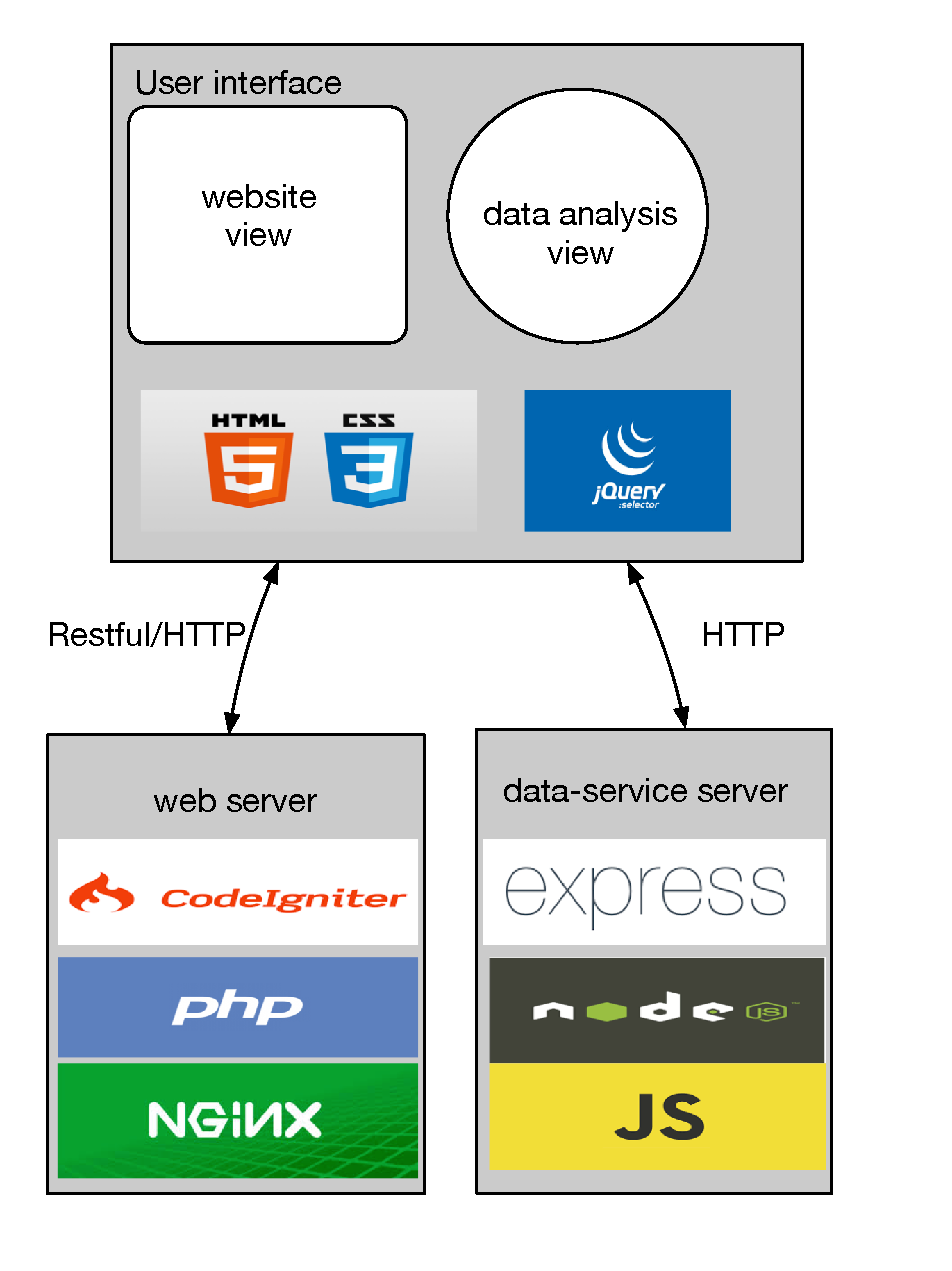
\includegraphics[width = 0.8\textwidth]{fig/layer-structure-overview.eps}
    \caption{layer structure overview}
    \label{fig:layer-overview}
\end{figure}

\subsection{Website MVC Design Pattern}
MVC (Model-View-Controller) is a kind of design patter in software engineering, it seperate application into three interconnected parts, model, controller, and view \cite{Leff2001} (see Figure \ref{fig:mvc}).
Controller act as the brain of application, dealing with users' request and converts requests into command for model and view.
View provides user a Graphical User Interface (GUI) to display application's state.
Model is the only one who can access data base directly, sometimes it represents a schema of table or specification or the data type.

\begin{figure}[H]
    \centering
    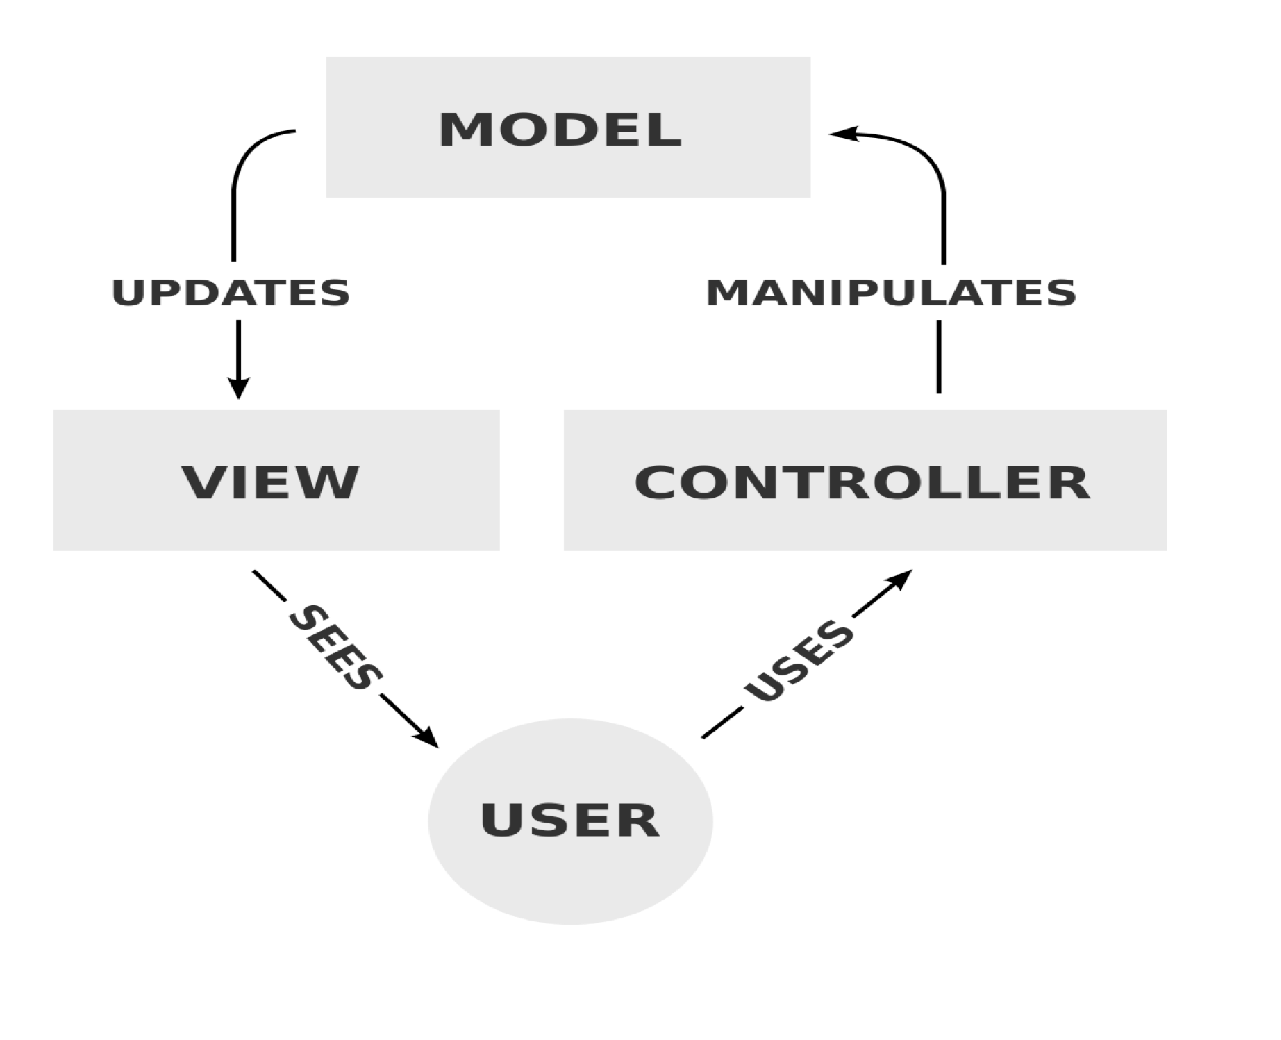
\includegraphics[width = 0.6\textwidth]{fig/mvc-relation.eps}
    \caption{Collaboration of MVC elements}
    \label{fig:mvc}
\end{figure}

\subsection{Activity Modules}
User activity datas play an important role in the proposed system, in order to analyze user's activity pattern when learning on websit we designed four activity module for different scenario (see Figure \ref{fig:act-module}) each activity module composed of multiple action which maps to user's activity.
First, account module records user's log into and logout from the website.
Second, page module records user's trail since he/she log in to the website, every record is tagged with ``leav'' or ``access'' to note action that triggered the record so that we can monitor user's web page activity.
Third, forum module has three action, ``post'', will records user's forum post, ``reply'' records which user give another postser a reply and ``like'' records user click like button on specific post and reply.
Finally, video module is the most complecated module among activity modules, ``play'', ``pause'', ``seek'', ``change rate'' are actions that user interacts with player, and ``leave when pause'', ``leave when play'' are actions that user leave the lecture video page.
\begin{figure}[H]
    \centering
    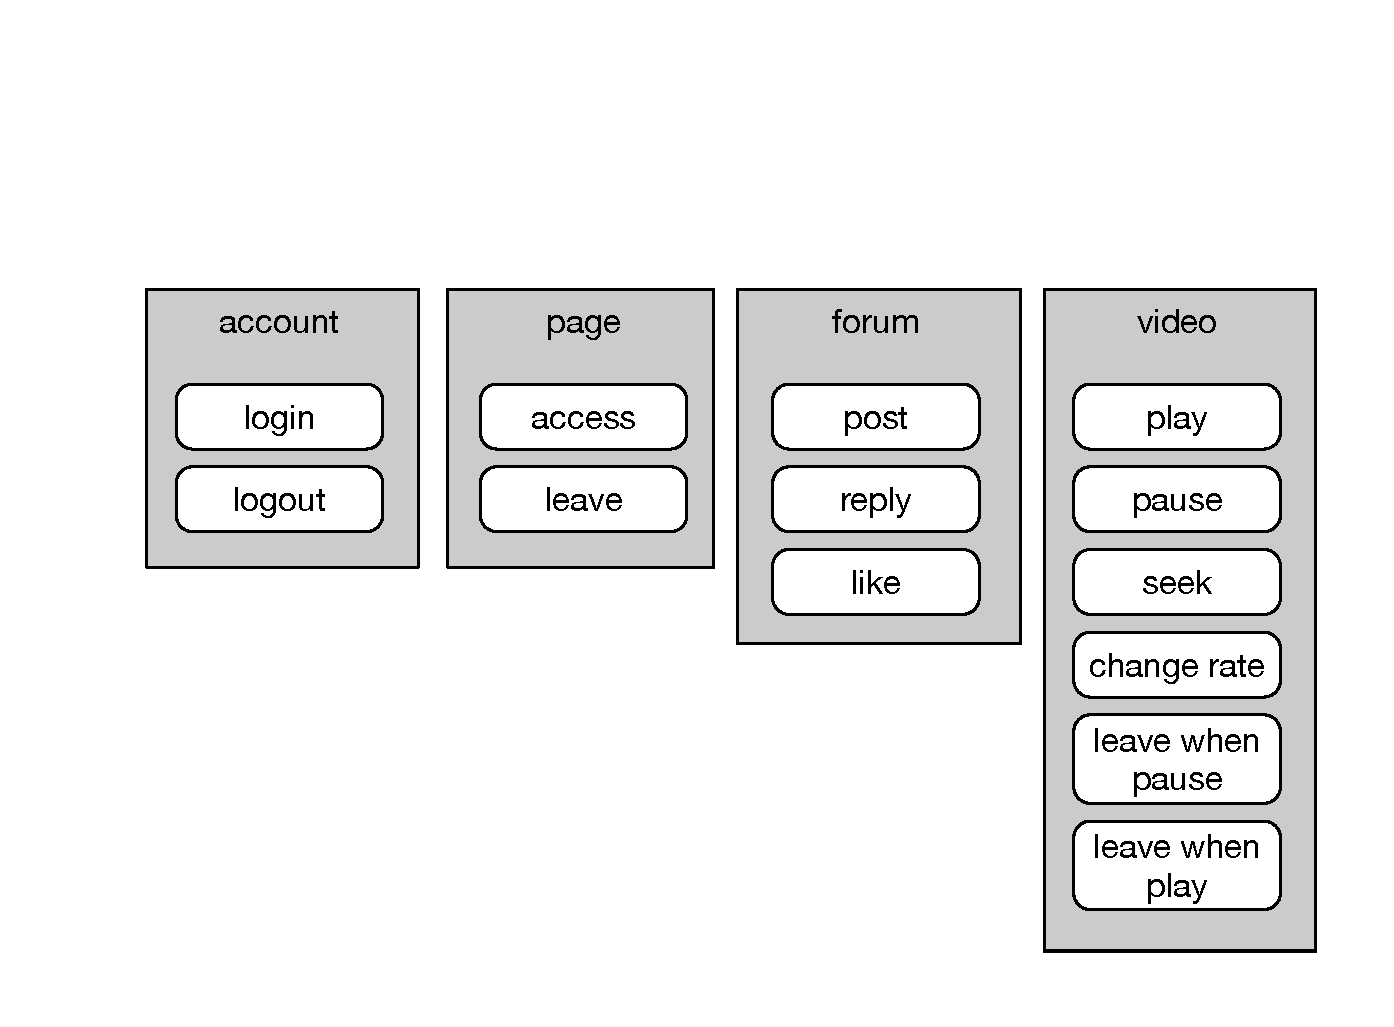
\includegraphics[width = 0.8\textwidth]{fig/activity-module.eps}
    \caption{User activity modules}
    \label{fig:act-module}
\end{figure}

\section{System Architecture}
Figure \ref{fig:sys-arch} illustrates the system architecture, which shows the detail tn each parts.
The whole system is constructured from two subsystem, web server and data-service system, these two system are run independently.
Web server is a entry for user to get access to this system, throug the browser user makes requests to web server to get pages they want;
moreover it contains the most logic of web application and responsible for front-end presentation to the user.
Data-service server is a pure API-server without front-end views, which responsible for collecting user activity datas and analyze collected datas.
Whenever users interact with view element such as click buttom, click play on website embedded player, leave pages, etc. on the views provided by web servers (website view in Figure \ref{fig:layer-overview}),
a data will be sent to data-service server as a record.
After every period of time, the data in data-service server will be analyzed by our algorithm and generate refined data.
Finally, we send back the refined data back to user interface at the time users call the related api on data-service, the browser will render the result based on refined data (data analysis view in Figure \ref{fig:layer-overview}).

\begin{figure}[H]
    \centering
    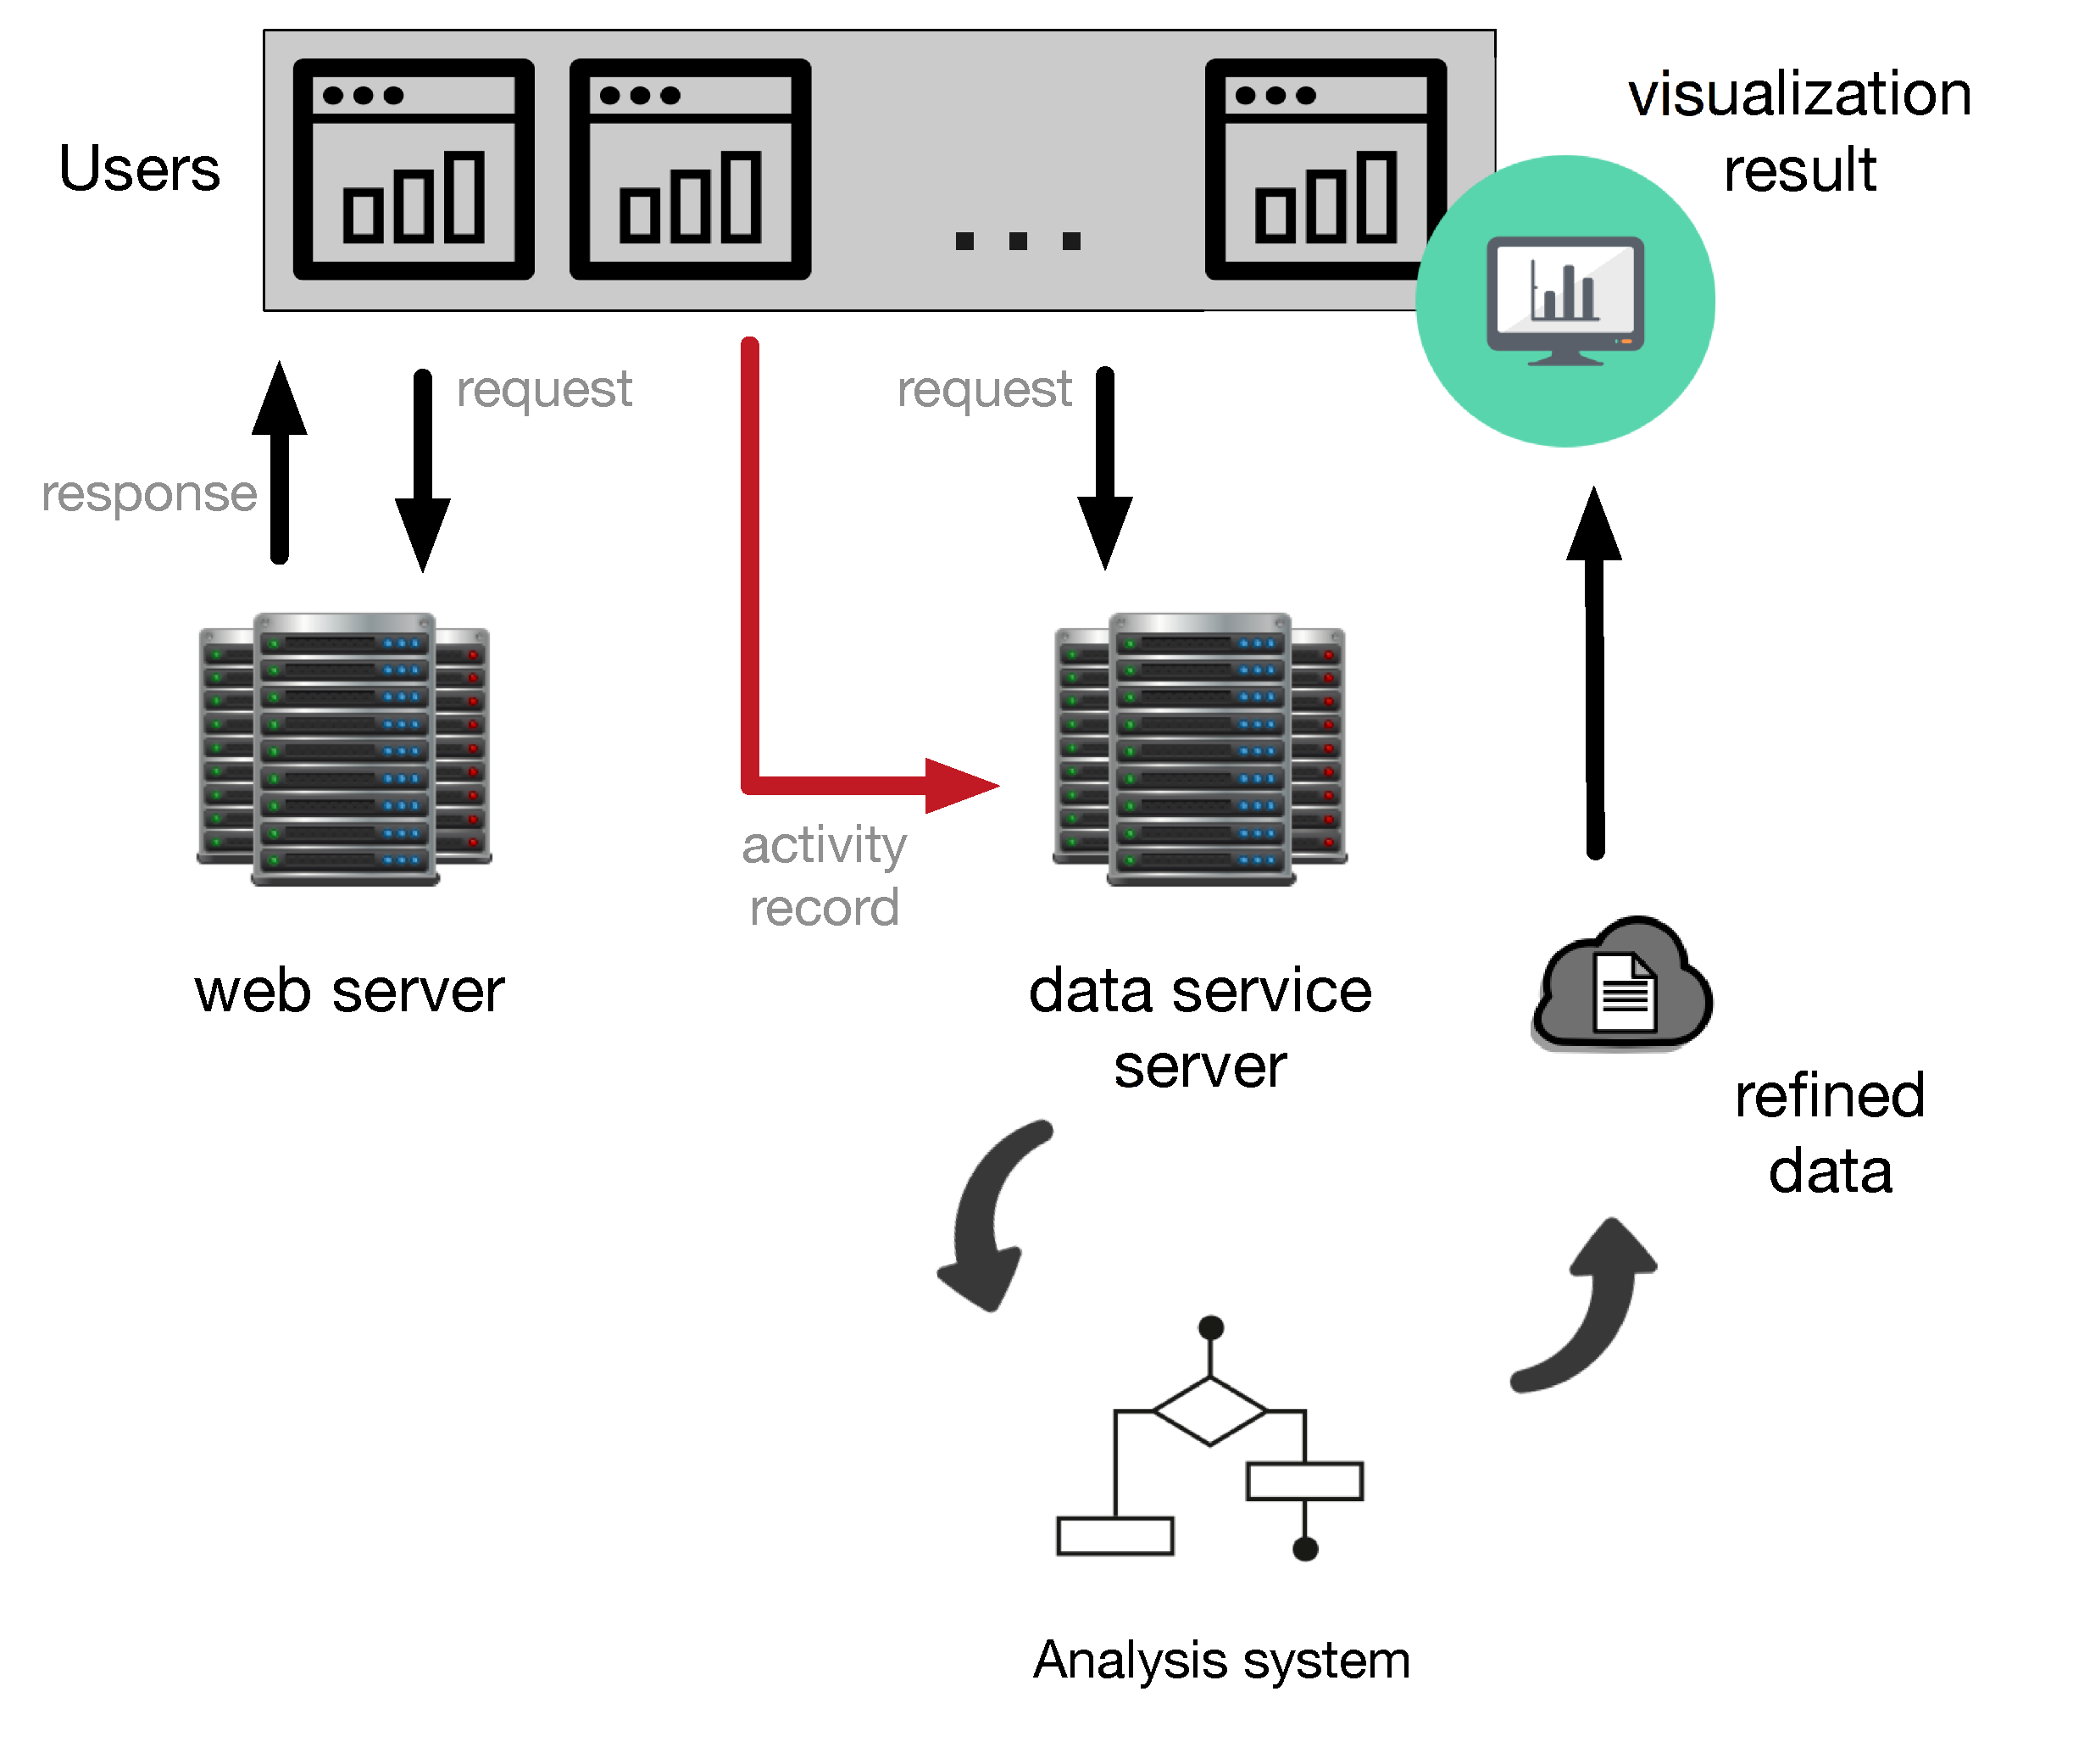
\includegraphics[width = 0.8\textwidth]{fig/system-architecture-outline.eps}
    \caption{system architecture}
    \label{fig:sys-arch}
\end{figure}

\section{Course Data Flow}
On MOOCs, there are two course starting models can be seen, one is course that had open before and reopen, which is old course, the other is new course that never opened before.
In view of keeping presented data updated, system should store refined data for user to access and simutaniously store new data for future analysis, to do so, we design two data flow for two different starting model.
To begin with, data flow of new course (see Figure \ref{fig:new-course-flow}) focus on maintaining a schema for system easy to store and be scerialized.
Moreover, to make system runs as a automation process we setup a worker to send a request to update datas to data-service server every period of time.

\begin{figure}[H]
    \centering
    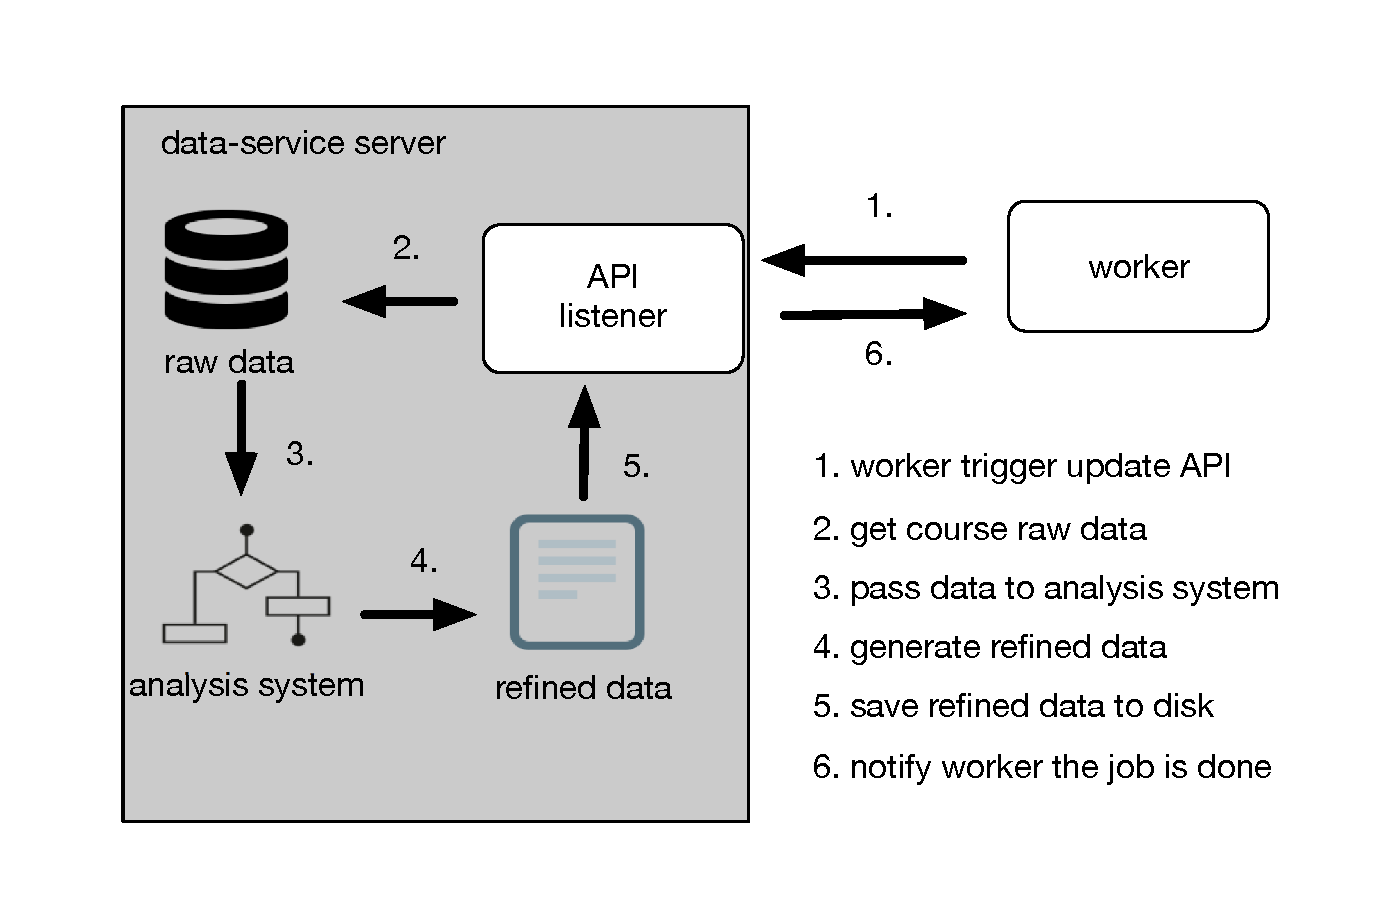
\includegraphics[width = 0.8\textwidth]{fig/new-class-workflow.eps}
    \caption{new course data work flow}
    \label{fig:new-course-flow}
\end{figure}

For new course that had never opened before (see Figure \ref{fig:new-course-flow}), we simply query the data base and send the return data to analysis system and then generate and store back the new refined data to replace the old one.

\begin{figure}[H]
    \centering
    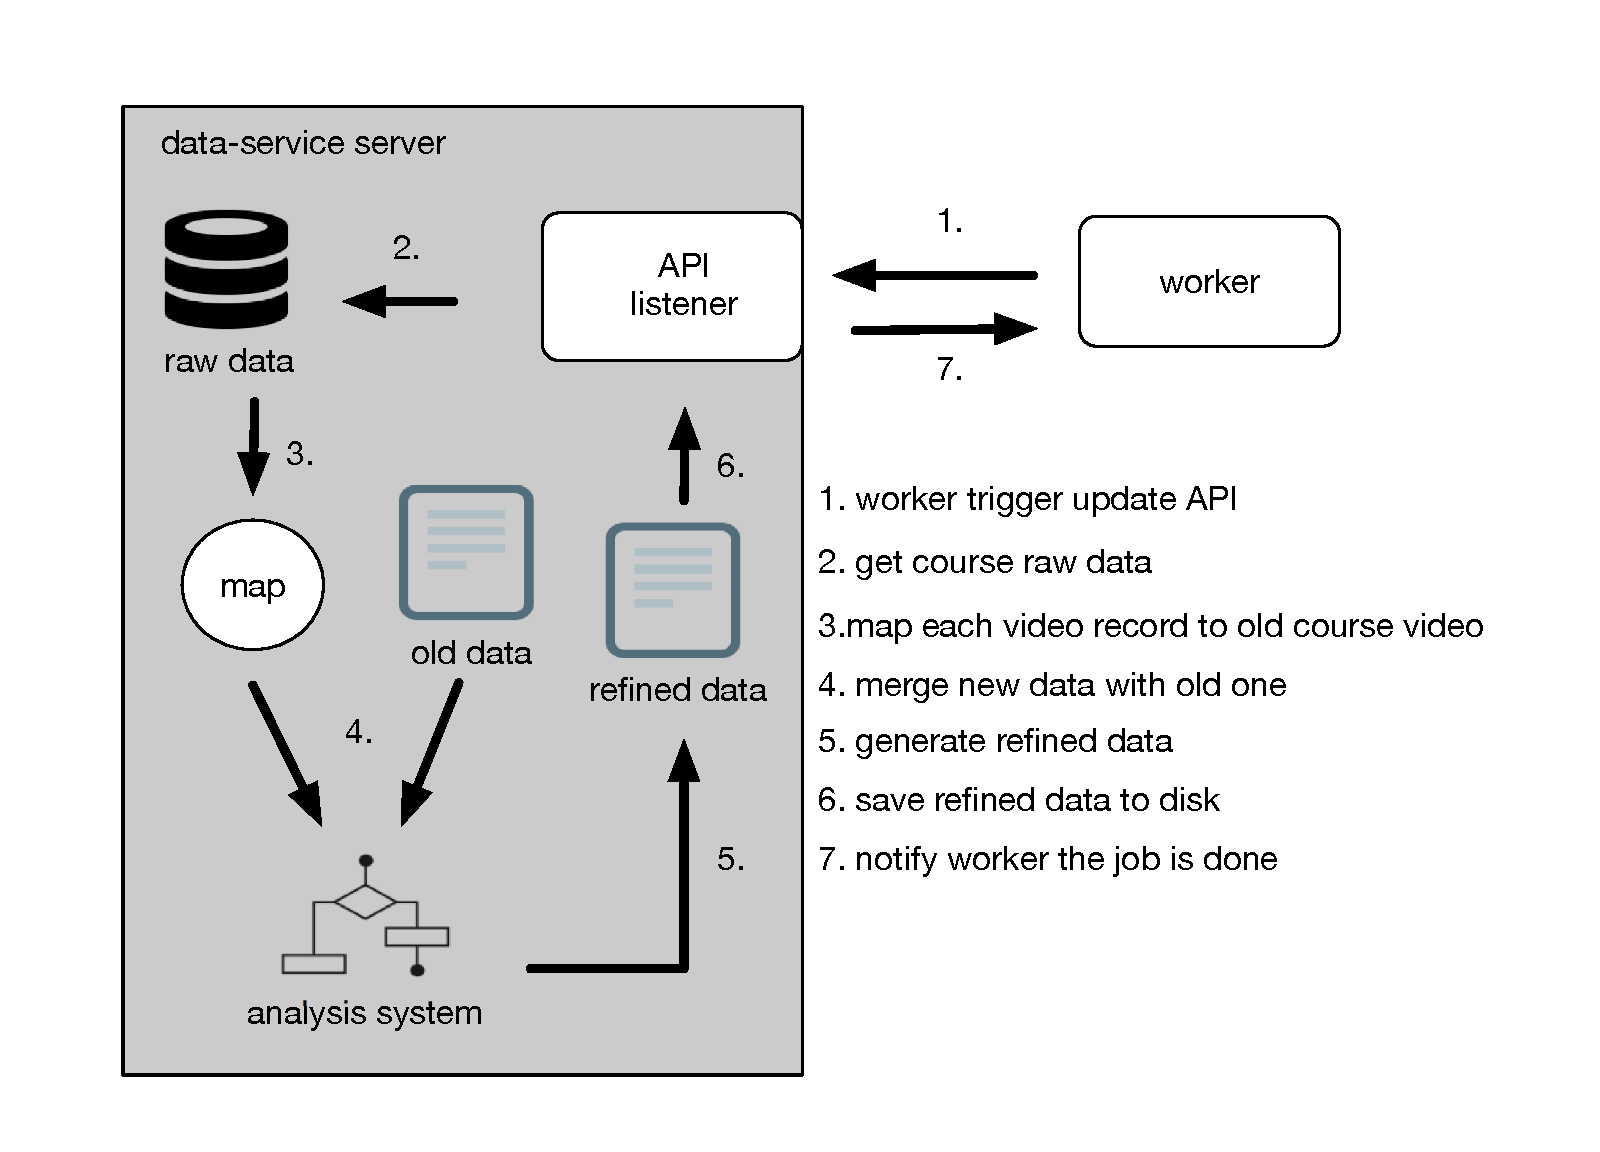
\includegraphics[width = 0.8\textwidth]{fig/old-course-flow.eps}
    \caption{old course data work flow}
    \label{fig:old-course-flow}
\end{figure}

On the other hand, processes to generate refined data for old courses is more complecated (see Figure \ref{fig:old-course-flow}), the challenge of the scenario is derive from data structure of MOOC platform, since there is no inherited relationship between courses.
To solve this issue, we maintain a map table for classes that have inherited relationship to map each lecture video in the course, so that we can merge the old course data with new one.
